\documentclass[11pt,landscape]{article}
\usepackage{tikz}
\usetikzlibrary{arrows, arrows.meta}
\usepackage[utf8]{inputenc}
\usepackage{amsfonts}
\usepackage{mathptmx}
\usepackage{float}
\usepackage{graphicx}
\usepackage{hyperref}
\usepackage{setspace}
\usepackage[normalem]{ulem}
\usepackage{linguex}
\usepackage[document]{ragged2e}
\usepackage{fancyhdr}
\usepackage[left=1cm,right=1cm,top=2.5cm,bottom=2.5cm]{geometry}
\usepackage{gb4e}
\author{Semih Can Aktepe}
\title{\vspace{-3cm}COGS543 Assignment 3}

\spacing{1.5}

\pagestyle{fancy}
\fancyhf{}
\lhead{Semih Can Aktepe}
\rhead{\today}
\cfoot{\thepage}

\begin{document}\thispagestyle{empty}
\maketitle
\justify
\noindent \textbf{Question 1:}\\

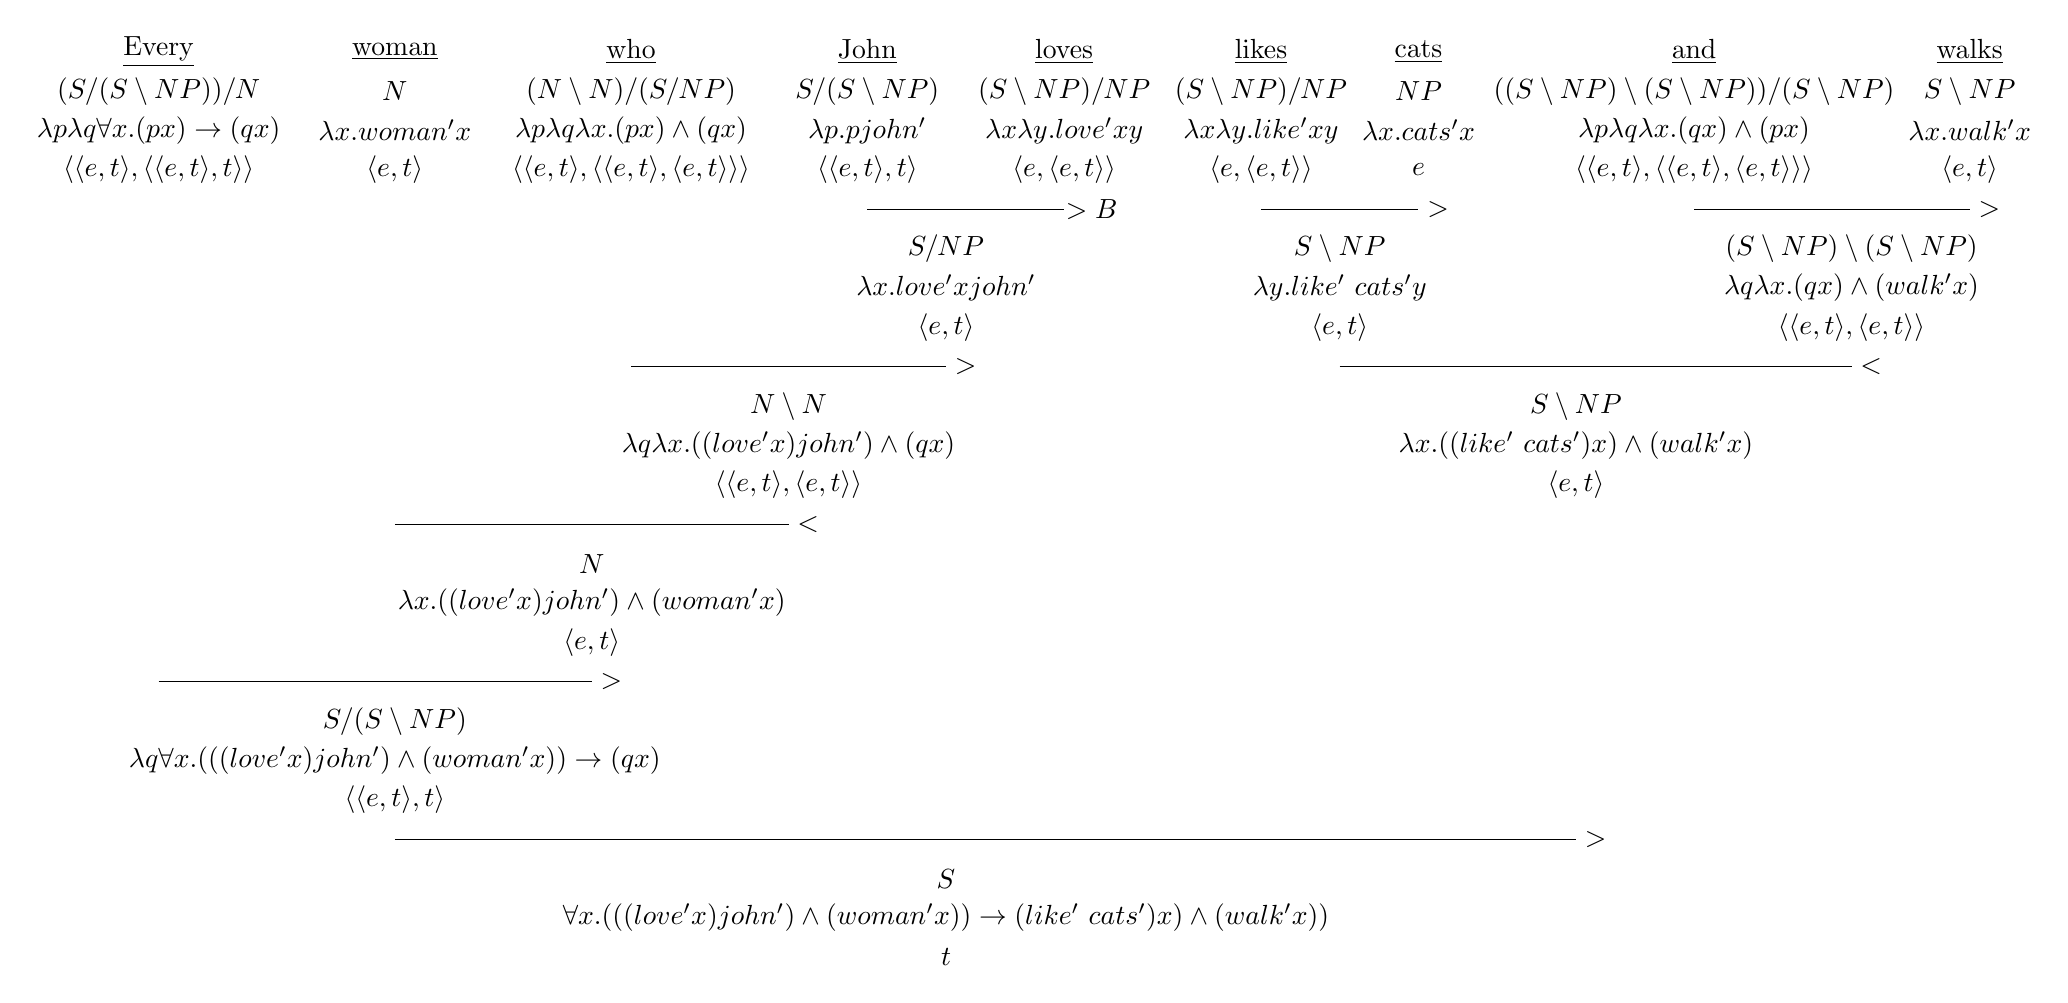
\begin{tikzpicture}
%Units of the sentence
\node at (0,0){\underline{Every}};
\node at (3,0){\underline{woman}};
\node at (6,0){\underline{who}};
\node at (9,0){\underline{John}};
\node at (11.5,0){\underline{loves}};
\node at (14,0){\underline{likes}};
\node at (16,0){\underline{cats}};
\node at (19.5,0){\underline{and}};
\node at (23,0){\underline{walks}};

%Syntactic categories
\node at (0,-0.5){$(S/(S\setminus NP))/N$};
\node at (3,-0.5){$N$};
\node at (6,-0.5){$(N\setminus N)/(S/NP)$};
\node at (9,-0.5){$S/(S\setminus NP)$};
\node at (11.5,-0.5){$(S\setminus NP)/NP$};
\node at (14,-0.5){$(S\setminus NP)/NP$};
\node at (16,-0.5){$NP$};
\node at (19.5,-0.5){$((S\setminus NP)\setminus(S\setminus NP))/(S\setminus NP)$};
\node at (23,-0.5){$S\setminus NP$};

%Semantic categories
\node at (0,-1){$\lambda p\lambda q\forall x.(px) \rightarrow (qx)$};
\node at (3,-1){$\lambda x.woman' x$};
\node at (6,-1){$\lambda p \lambda q \lambda x. (px) \wedge (qx)$};
\node at (9,-1){$\lambda p.p john'$};
\node at (11.5,-1){$\lambda x \lambda y. love' xy$};
\node at (14,-1){$\lambda x \lambda y. like' xy$};
\node at (16,-1){$\lambda x.cats' x$};
\node at (19.5,-1){$\lambda p \lambda q \lambda x. (qx) \wedge (px)$};
\node at (23,-1){$\lambda x. walk' x$};

%Semantic types
\node at (0,-1.5){$\langle\langle e,t\rangle,\langle\langle e,t\rangle, t\rangle\rangle$};
\node at (3,-1.5){$\langle e,t\rangle$};
\node at (6,-1.5){$\langle\langle e,t\rangle,\langle \langle e,t\rangle, \langle e,t\rangle\rangle\rangle$};
\node at (9,-1.5){$\langle\langle e,t\rangle, t\rangle$};
\node at (11.5,-1.5){$\langle e, \langle e,t\rangle\rangle$};
\node at (14,-1.5){$\langle e, \langle e,t\rangle\rangle$};
\node at (16,-1.5){$e$};
\node at (19.5,-1.5){$\langle\langle e,t\rangle,\langle\langle e,t\rangle,\langle e,t\rangle\rangle\rangle$};
\node at (23,-1.5){$\langle e,t\rangle$};

%Merge of John and loves
\draw (9,-2)--(11.5,-2);\node at (11.85,-2){$>B$};
\node at (10,-2.5){$S/NP$};
\node at (10,-3){$\lambda x. love' x john'$};
\node at (10,-3.5){$\langle e,t\rangle$};

%Merge of likes and cats
\draw (14,-2)--(16,-2);\node at (16.25,-2){$>$};
\node at (15,-2.5){$S\setminus NP$};
\node at (15,-3){$\lambda y. like'$ $cats' y$};
\node at (15,-3.5){$\langle e,t\rangle$};

%Merge of and and walks
\draw (19.5,-2)--(23,-2);\node at (23.25,-2){$>$};
\node at (21.5,-2.5){$(S\setminus NP)\setminus (S\setminus NP)$};
\node at (21.5,-3){$\lambda q\lambda x.(qx) \wedge (walk' x)$};
\node at (21.5,-3.5){$\langle\langle e,t\rangle, \langle e,t\rangle\rangle$};

%Merge of who and John
\draw (6,-4)--(10,-4);\node at (10.25,-4){$>$};
\node at (8,-4.5){$N\setminus N$};
\node at (8,-5){$\lambda q\lambda x.((love'x)john') \wedge (q x)$};
\node at (8,-5.5){$\langle\langle e,t\rangle, \langle e,t\rangle\rangle$};

%Merge of likes cats and walks
\draw (15,-4)--(21.5,-4);\node at (21.75,-4){$<$};
\node at (18,-4.5){$S\setminus NP$};
\node at (18,-5){$\lambda x.((like'$ $cats')x) \wedge (walk' x)$};
\node at (18,-5.5){$\langle e,t\rangle$};

%Merge of woman and who
\draw (3,-6)--(8,-6);\node at (8.25,-6){$<$};
\node at (5.5,-6.5){$N$};
\node at (5.5,-7){$\lambda x.((love'x)john') \wedge (woman' x)$};
\node at (5.5,-7.5){$\langle e,t\rangle$};

%Merge of every and woman
\draw (0,-8)--(5.5,-8);\node at (5.75,-8){$>$};
\node at (3,-8.5){$S/(S\setminus NP)$};
\node at (3,-9){$\lambda q\forall x.(((love'x)john') \wedge (woman' x))\rightarrow (qx)$};
\node at (3,-9.5){$\langle\langle e,t\rangle, t\rangle$};

%Merge of every woman who John loves and likes cats and walks
\draw (3,-10)--(18,-10);\node at (18.25,-10){$>$};
\node at (10,-10.5){$S$};
\node at (10,-11){$\forall x.(((love'x)john') \wedge (woman' x))\rightarrow (like'$ $cats') x) \wedge (walk' x))$};
\node at (10,-11.5){$t$};


\end{tikzpicture}
\clearpage
\noindent \textbf{Question 2:}\\

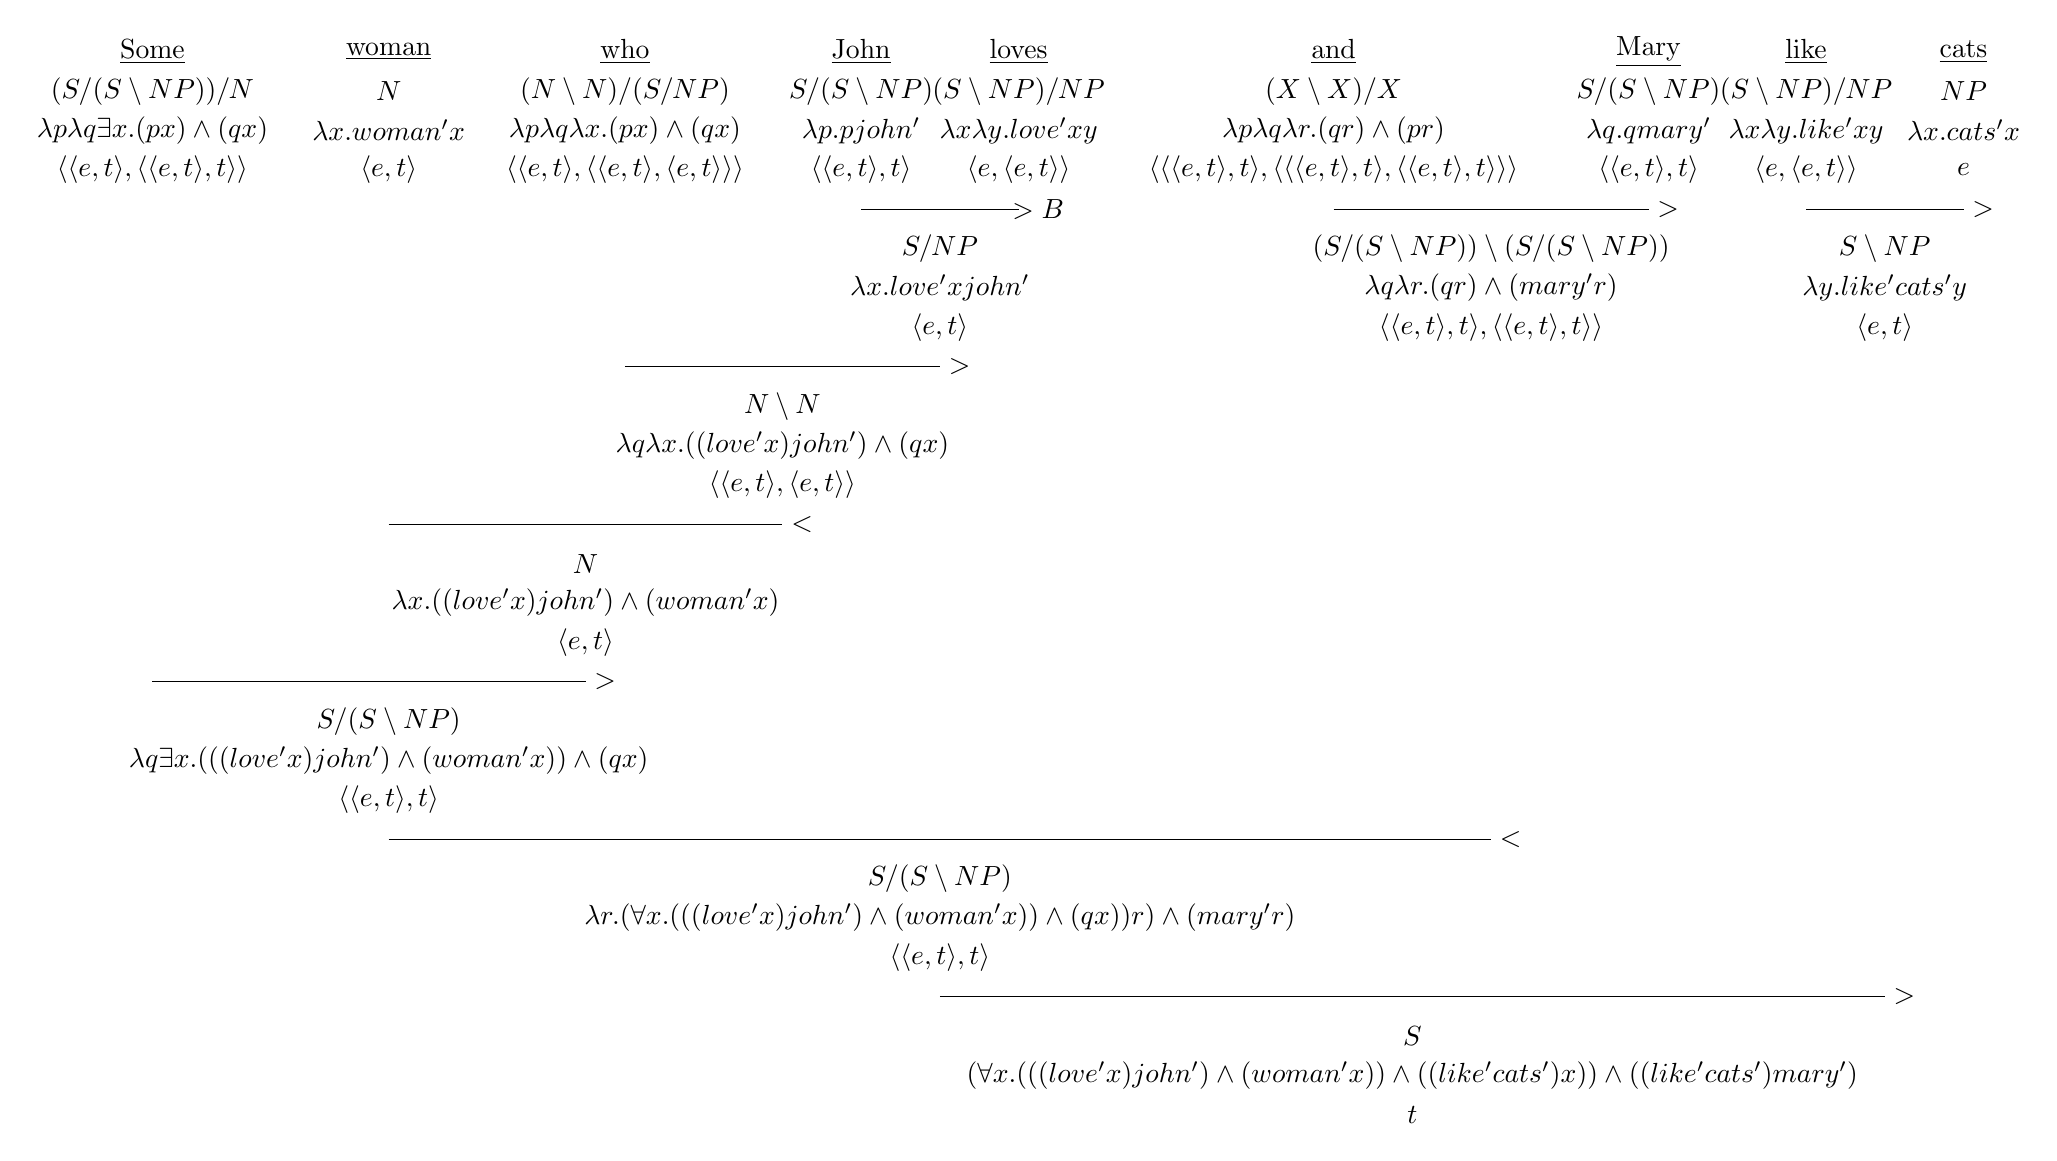
\begin{tikzpicture}
%Units of the sentence
\node at (0,0){\underline{Some}};
\node at (3,0){\underline{woman}};
\node at (6,0){\underline{who}};
\node at (9,0){\underline{John}};
\node at (11,0){\underline{loves}};
\node at (15,0){\underline{and}};
\node at (19,0){\underline{Mary}};
\node at (21,0){\underline{like}};
\node at (23,0){\underline{cats}};

%Syntactic categories
\node at (0,-0.5){$(S/(S\setminus NP))/N$};
\node at (3,-0.5){$N$};
\node at (6,-0.5){$(N\setminus N)/(S/NP)$};
\node at (9,-0.5){$S/(S\setminus NP)$};
\node at (11,-0.5){$(S\setminus NP)/NP$};
\node at (15,-0.5){$(X\setminus X)/X$};
\node at (19,-0.5){$S/(S\setminus NP)$};
\node at (21,-0.5){$(S\setminus NP)/NP$};
\node at (23,-0.5){$NP$};

%Semantic categories
\node at (0,-1){$\lambda p\lambda q\exists x.(px) \wedge (qx)$};
\node at (3,-1){$\lambda x.woman' x$};
\node at (6,-1){$\lambda p \lambda q \lambda x. (px) \wedge (qx)$};
\node at (9,-1){$\lambda p.p john'$};
\node at (11,-1){$\lambda x \lambda y. love' xy$};
\node at (15,-1){$\lambda p\lambda q\lambda r.(qr)\wedge (pr)$};
\node at (19,-1){$\lambda q. q mary'$};
\node at (21,-1){$\lambda x \lambda y. like' xy$};
\node at (23,-1){$\lambda x.cats' x$};

%Semantic types
\node at (0,-1.5){$\langle\langle e,t\rangle,\langle\langle e,t\rangle, t\rangle\rangle$};
\node at (3,-1.5){$\langle e,t\rangle$};
\node at (6,-1.5){$\langle\langle e,t\rangle,\langle \langle e,t\rangle, \langle e,t\rangle\rangle\rangle$};
\node at (9,-1.5){$\langle\langle e,t\rangle, t\rangle$};
\node at (11,-1.5){$\langle e, \langle e,t\rangle\rangle$};
\node at (15,-1.5){$\langle\langle\langle e,t\rangle, t\rangle,\langle\langle\langle e,t\rangle, t\rangle,\langle\langle e,t\rangle, t\rangle\rangle\rangle$};
\node at (19,-1.5){$\langle\langle e,t\rangle, t\rangle$};
\node at (21,-1.5){$\langle e, \langle e,t\rangle\rangle$};
\node at (23,-1.5){$e$};

%Merge of John and loves
\draw (9,-2)--(11,-2);\node at (11.25,-2){$>B$};
\node at (10,-2.5){$S/NP$};
\node at (10,-3){$\lambda x. love' x john'$};
\node at (10,-3.5){$\langle e,t\rangle$};

%Merge of and and Mary
\draw (15,-2)--(19,-2);\node at (19.25,-2){$>$};
\node at (17,-2.5){$(S/(S\setminus NP))\setminus (S/(S\setminus NP))$};
\node at (17,-3){$\lambda q\lambda r. (qr)\wedge (mary'r)$};
\node at (17,-3.5){$\langle\langle e,t\rangle, t\rangle,\langle\langle e,t\rangle,t\rangle\rangle$};

%Merge of likes and cats
\draw (21,-2)--(23,-2);\node at (23.25,-2){$>$};
\node at (22,-2.5){$S\setminus NP$};
\node at (22,-3){$\lambda y. like'cats' y$};
\node at (22,-3.5){$\langle e,t\rangle$};

%Merge of who and John
\draw (6,-4)--(10,-4);\node at (10.25,-4){$>$};
\node at (8,-4.5){$N\setminus N$};
\node at (8,-5){$\lambda q\lambda x.((love'x)john') \wedge (q x)$};
\node at (8,-5.5){$\langle\langle e,t\rangle, \langle e,t\rangle\rangle$};

%Merge of woman and who
\draw (3,-6)--(8,-6);\node at (8.25,-6){$<$};
\node at (5.5,-6.5){$N$};
\node at (5.5,-7){$\lambda x.((love'x)john') \wedge (woman' x)$};
\node at (5.5,-7.5){$\langle e,t\rangle$};

%Merge of some and woman
\draw (0,-8)--(5.5,-8);\node at (5.75,-8){$>$};
\node at (3,-8.5){$S/(S\setminus NP)$};
\node at (3,-9){$\lambda q\exists x.(((love'x)john') \wedge (woman' x))\wedge (qx)$};
\node at (3,-9.5){$\langle\langle e,t\rangle, t\rangle$};

%Merge of some woman who John loves and Mary
\draw (3,-10)--(17,-10);\node at (17.25,-10){$<$};
\node at (10,-10.5){$S/(S\setminus NP)$};
\node at (10,-11){$\lambda r.(\forall x.(((love'x)john') \wedge (woman' x))\wedge (qx))r) \wedge (mary' r)$};
\node at (10,-11.5){$\langle\langle e,t\rangle, t\rangle$};

%Final Merge
\draw (10,-12)--(22,-12);\node at (22.25,-12){$>$};
\node at (16,-12.5){$S$};
\node at (16,-13){$(\forall x.(((love'x) john') \wedge (woman' x)) \wedge ((like' cats') x)) \wedge ((like' cats') mary')$};
\node at (16,-13.5){$t$};


\end{tikzpicture}
\vspace{1cm}
\noindent and = $((S/(S\setminus NP))\setminus (S/(S\setminus NP)))/(S/(S\setminus NP))$






















\end{document}